\label{section:1d_column_example}
This example \texttt{1\_VSF\_Column} simulates variably-saturated flow in a 1D column of homogeneous sand 100 cm thick using the following  parameter values:

\begin{center}
    \begin{tabular}{lll}  \hline
        Parameter                               & Value & Unit                           \\ \hline
        Specific yield (porosity)               &  0.43                    &             \\
        Vertical hydraulic conductivity         &  $ 10$                   & cm d$^{-1}$  \\
        Horizontal hydraulic conductivity       &  $ 1 \times 10^{-5}$     & cm d$^{-1}$  \\
        Specific storage coefficient            &  $ 1 \times 10^{-7}$     & cm$^{-1}$   \\
        Van Genuchten Alpha                     &  $ 3.6 \times 10^{-2}$   & cm$^{-1}$     \\
        Van Genuchten Beta                      &  1.56                    &             \\
        Residual saturation                     &  0.1814                  &             \\
    \hline
    \end{tabular}
\end{center}

The Van Genuchten unsaturated function type was used.

A uniform rainfall of 0.4 cm/day was applied to the top of the column and the base was fixed at a pressure head of -100 cm.

An initial head was assigned as a function of $z$ (i.e. elevation) as: head=-100.0 cm at $z$=0.0 cm to head=0.0 cm at $z$=100.0 cm.

\pagebreak
Here is a comparison of pressure head (upper plot) and saturation (lower plot) versus elevation results for  \mfus\ and \hgs(\textbf{\sf HGS}) at 20 and 40 days:

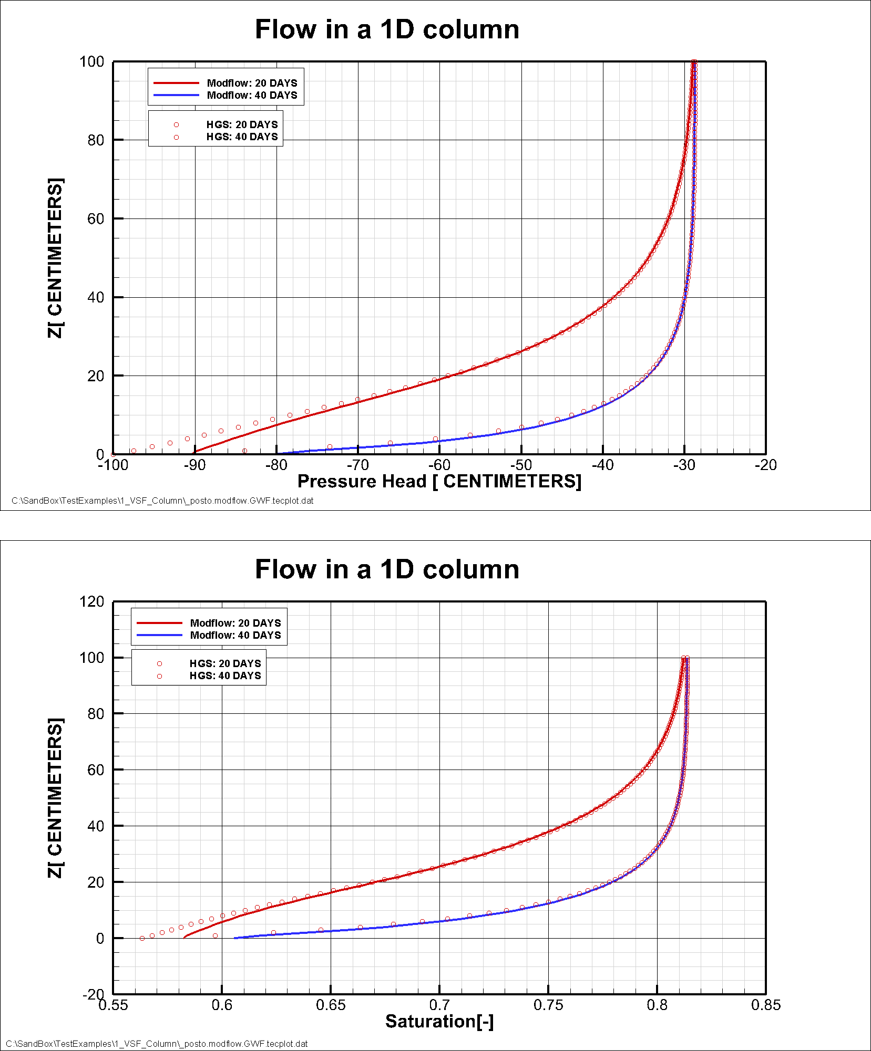
\includegraphics[width=0.87\textwidth]{5_1_1d_combined}

The two models yield very similar results except near the base of the column.

    \pagebreak
Just as a demonstration, a second simulation \texttt{1\_VSF\_Column\_Brooks} was carried out using the   Brooks-Corey unsaturated function type,  with a Brooks-Corey exponent of 6.5714.  Here is a plot of pressure head (upper plot) and saturation (lower plot) versus elevation results  \mfus\ at 20 and 40 days:

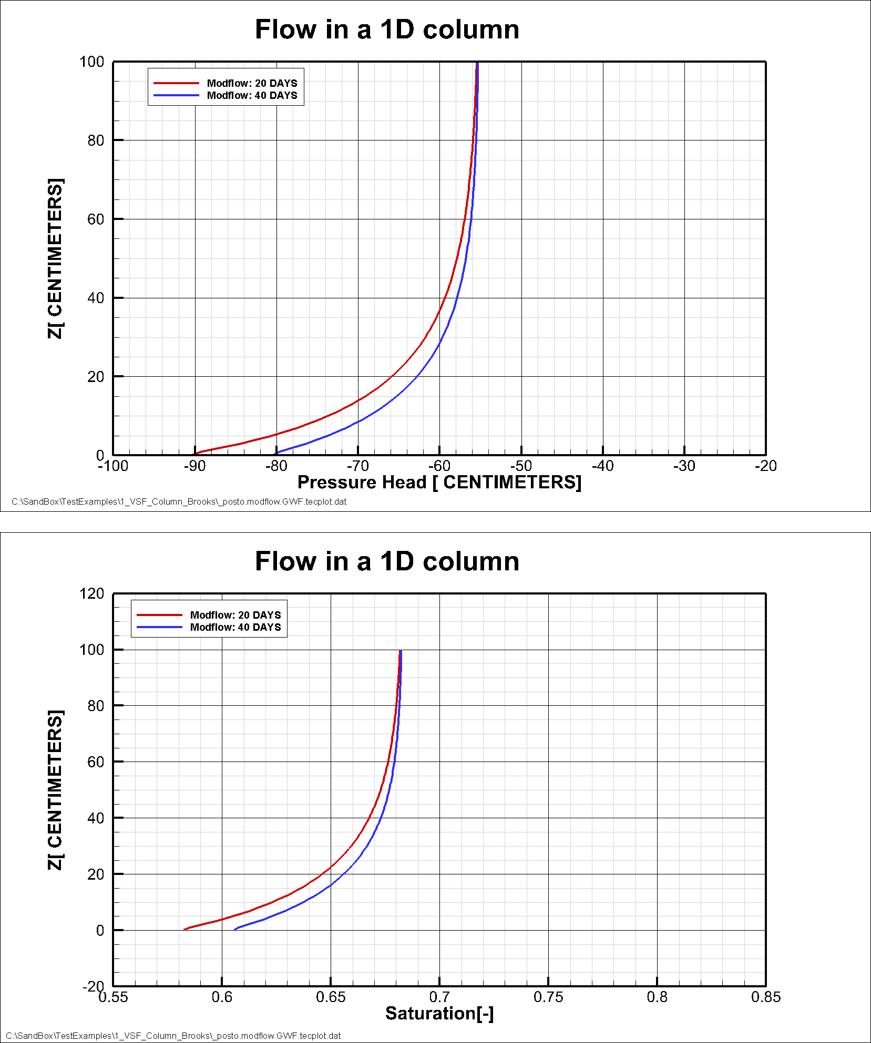
\includegraphics[width=0.87\textwidth]{5_2_1d_combined_Brooks}
